\chapter{Fundamental Algorithms}
\label{chap:fundamental_algorithms}

\begin{figure}[ht]
	\hfill
	\begin{minipage}{0.5\textwidth}
		\centering
		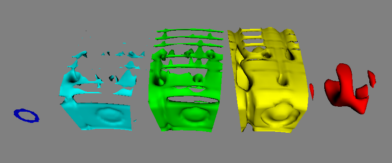
\includegraphics{VTKTextbook-54}\\
		\caption*{\texttt{Isosurfaces of a combustor dataset computed at multiple values..}}
	\end{minipage}
\end{figure}

\firstletter{W}e have seen how to represent basic types of visualization data such as image data, structured grids, unstructured grids, and polygonal data.
This chapter explores methods to transform this data to and from these various representations, eventually generating graphics primitives that we can render.
These methods are called algorithms, and are of special interest to those working in the field of visualization.
Algorithms are the verbs that allow us to express our data in visual form.
By combining these verbs appropriately, we can reduce complex data into simple, readily comprehensible sentences that are the power of data visualization.

\section{Introduction}

The algorithms that transform data are the heart of data visualization.
To describe the various transformations available, we need to categorize algorithms according to the structure and type of transformation.
By structure we mean the effects that transformation has on the topology and geometry of the dataset.
By type we mean the type of dataset that the algorithm operates on.

Structural transformations can be classified in four ways, depending on how they affect the geometry, topology, and attributes of a dataset.

\section{Bibliographic Notes}

Color mapping is a widely studied topic in imaging, computer graphics, visualization, and human factors. References \cite{Durrett87} \cite{Ware88} \cite{Rheingans92} provide samples of the available literature. You also may want to learn about the physiological and psychological effects of color on perception. The text by Wyszecki and Stiles \cite{Wyszecki82} serves as an introductory reference.

Contouring is a widely studied technique in visualization because of its importance and popularity. Early techniques were developed for 2D data \cite{Watson92}. Three-dimensional techniques were developed initially as contour connecting methods \cite{Fuchs77} --- that is, given a series of 2D contours on evenly spaced planes, connect the contours to create a closed surface. Since the introduction of marching cubes \cite{Lorensen87}, many other techniques have been implemented. (A few of these include \cite{Nielson91} \cite{Montani94} and \cite{Durst88} ). A particularly interesting reference is given by Livnat et al. \cite{Livnat96}. They show a contouring method with the addition of a preprocessing step that generates isocontours in near optimal time.

Although we barely touched the topic, the study of chaos and chaotic vibrations is a delightfully interesting topic. Besides the original paper by Lorenz \cite{Lorenz63}, the book by Moon \cite{Moon87} is a good place to start.

Two- and three-dimensional vector plots have been used by computer analysts for many years \cite{Fuller80}. Streamlines and streamribbons also have been applied to the visualization of complex flows \cite{Volpe89}. Good general references on vector visualization techniques are given in \cite{Helman90} and \cite{Richter90}.

Tensor visualization techniques are relatively few in number. Most techniques are glyph oriented \cite{Haber90} \cite{deLeeuw93}. We will see a few more techniques in Chapter 9.

Blinn \cite{Blinn82}, Bloomental \cite{Bloomenthal88} \cite{Bloomenthal97} and Wyvill \cite{Wyvill86} have been important contributors to implicit modeling. Implicit modeling is currently popular in computer graphics for modeling "soft" or "blobby" objects. These techniques are simple, powerful, and are becoming widely used for advanced computer graphics modeling.


\printbibliography


\section{Exercises}
\begin{enumerate}

\item Sketch contour cases for marching triangles. How many cases are there?

\item Sketch contour cases for marching tetrahedron. How many cases are there?

\item A common visualization technique is to animate isosurface value. The procedure is to smoothly vary isosurface value over a specified range.	
\begin{enumerate}
	\item Create an animation sequence for the quadric example ( **Figure4--1** )
	\item Create an animation sequence for the head sequence ( **Figure6-11** (b))
\end{enumerate}

\item Marching Cubes visits each cell during algorithm execution. Many of these cells do not contain the isosurface. Describe a technique to improve the performance of isosurface extraction by eliminating visits to cells not containing isosurface. ( *Hint:* use a preprocessing step to analyze data. Assume that many isosurfaces will be extracted and that the preprocessing step will not count against execution time.)

\item Scanline rasterization proceeds along horizontal spans in graphics hardware (see tion" on page54 ). Interpolation of color occurs along horizontal spans as well.
\begin{enumerate}
	\item Show how the orientation of a polygon affects interpolated color.
	\item Discuss potential problems caused by orientation dependent viewing of visualizations.
\end{enumerate}

\item Write a program to simulate beam vibration. Use the code associated with **Figure6-14** (a) as your starting point.

\item 	 Using the filters vtkStreamLine, vtkMaskPoints, and vtkGlyph3D, create a visualization consisting of oriented glyphs along a streamline.

\item Visualize the following functions.
\begin{enumerate}
	\item Scalar $S(x,y,z)=sin(xy)$ for $x,y$, between $0$ and $\pi$.
	\item The effective stress field (a scalar field) from **Figure6–21**.
	\item The vector field described in the combustor data (i.e., combq.bin and combxyz.bin ).
\end{enumerate}

\item Tensor ellipsoids are based on an ellipsoidal glyph. Describe two other glyphs that you might use.

\item Write a source object to generate a polygonal representation of a torus.

\item Design a glyph to convey airplane heading, speed, and altitude, and proximity (i.e., distance) to other planes.

\item Morphing is a process to smoothly blend images (2D) or geometry (3D) between two known images or geometry. Using an implicit modeling approach, how would you morph a torus into a cube?

\item Describe a technique to visualize vector information by animating a color map. (emph{Hint:} By choosing a map carefully, you can give the illusion of motion across a surface.)

\item Isoline contours of different values are typically shown together in one image.
\begin{enumerate}
	\item Describe the advantages and disadvantages of displaying isosurfaces simultaneously.
	\item What two graphics properties might you adjust to improve the display of multiple isosurefaces?
\end{enumerate}

\item Describe a parallel algorithm for marching cubes. Use a parallel architecture of your choice.

\item Decomposition can greatly increase the speed of an operation.
\begin{enumerate}
	\item  Prove that 3D Gaussian smoothing can be decomposed into three 1D operations.
	\item Give the complexity of the decomposed filter and the same filter implemented as a 3D convolution.
	\item Under what conditions can constant smoothing be decomposed into 1D operations.
\end{enumerate}

\end{enumerate}
